\documentclass{article}
\usepackage[brazil]{babel}
\usepackage{graphicx}
\usepackage[utf8]{inputenc}




\title{Economia para Empreendedor}
\author{Henrique Carvalho de Melo}
\date{Abril 2022}





\begin{document}

\maketitle

\begin{figure}[h!]
\centering

\includegraphics[width=0.8\textwidth]{empreendedor.png}
\caption{Ilustração de Empreendedorismo.} \cite{empreendedorismo}
\label{fig:Empreendedorismo}

\end{figure}





\section{Introdução}
\paragraph{}A disciplina de Economia para Empreendedor é uma cadeira eletiva do curso de Ciência da Computação que ensina os conceitos básicos de empreendedorismo e tem como função nortear os alunos que buscam empreender, mas não sabem como começar um negócio.\cite{dornelas2008empreendedorismo}




\section{Relevância}
\paragraph{} A cadeira de Economia para Empreendedor é de grande importância, não só para a área de computação, mas também para todas as áreas do conhecimento, pois com os conhecimentos da disciplina o estudante poderá futuramente criar um negócio mais bem-sucedido (Figura \ref{fig:Empreendedorismo}). \cite{leite2017fenomeno}
\paragraph{} No contexto atual a relevância dessa cadeira ainda aumenta, visto que a pandemia da Covid-19 trouxe ainda mais dificuldades para as empresas, tornando ainda mais necessário o conhecimento proporcionado pela matéria. 
\newline \cite{stangherlin2020desafios}



\section{Relações com outras disciplinas}
\paragraph{} A cadeira IF780 (Economia para Empreendedor) é uma disciplina eletiva, isto é, não obrigatória e que não precisa de nenhum pré-requisito para cursá-la. Além disso, para essa matéria,  também não é necessário pagar nenhuma cadeira acompanhada dela (co-requisito) e nem precisa de alguma carga horária específica, como pode ser visto na Figura \ref{fig:Ementa}. Apesar disso, não deixa de ser uma cadeira importantíssima não só para o curso de Ciência da Computação, mas também para qualquer curso que queira promover o empreendedorismo.




\begin{figure}[h!]
\centering
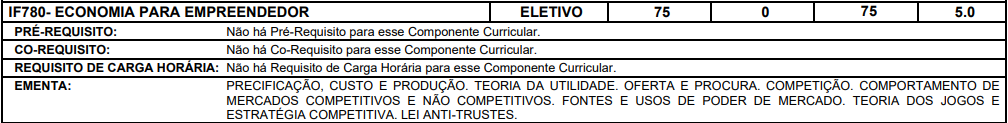
\includegraphics[width=1\textwidth]{ementa.png}
\caption{Ementa da Cadeira de Economia para Empreendedor}\cite{ementa}
\label{fig:Ementa}

\end{figure}

\bibliographystyle{apalike}
\bibliography{ref.bib}

\end{document}
